
\begin{figure*}[h!]
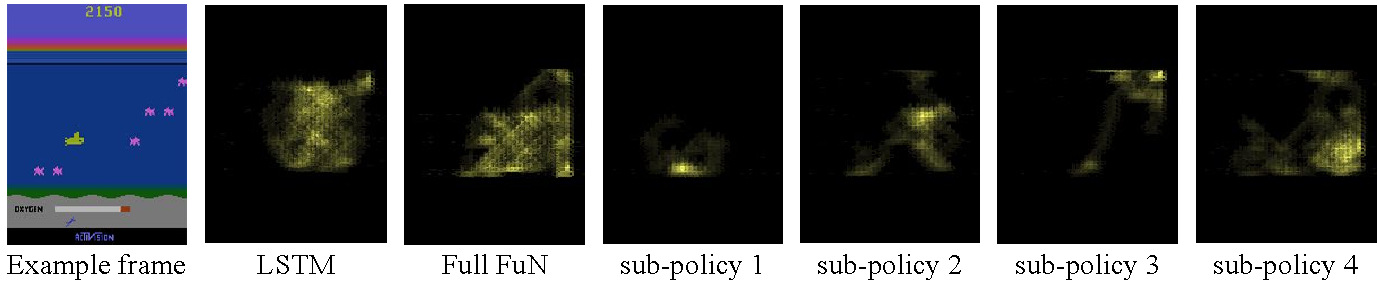
\includegraphics[scale=0.7]{./Figures/Seaquest_options.pdf}
  \caption{Visualisation of sub-policies learnt on sea quest game. We sample a random goal and feed it as a constant conditioning for the Worker and record its behaviour. We filter out only the image of the ship and average the frames, acquiring the heat-map of agents spatial location. From left to right: i) an example frame of the game ii) policy learnt by LSTM baseline iii) full policy learnt by FuN followed by set of different sub-policies. Notice how sub-policies are concentrated around different areas of the playable space. Sub-policy 3 is used to swim up for oxygen. \label{fig:SeaQ_subgoals} \figskiny }
\end{figure*}

\section{Experiments}
\seckiny
\label{sec:Experiments}



The goal of our experiments is to demonstrate that FuN learns non-trivial, helpful, and interpretable sub-policies and sub-goals, and also to validate components of the architecture. 
We start by describing technical details of the experimental setup and then present results on Montezuma's revenge -- an infamously hard ATARI game -- in section~\ref{subsec:Montezuma}. 
Section~\ref{subsec:atari} presents results on more ATARI games and extensively compares FuN to LSTM baseline with different discount factors and BPTT lengths.
In section~\ref{subsec:Mem_in_Lab} we present results on a set of visual memorisation tasks in 3D environment. 
Section~\ref{subsec:ablative} presents an ablation study of FuN, validating our design choices. 


\parskiny
\paragraph{Baseline.} Our main baseline is a recurrent LSTM network on top of a representation learned by a CNN. The LSTM~\cite{hochreiter1997lstm} architecture is a widely used recurrent network and it was demonstrated to perform very well on a suite of reinforcement learning problems~\cite{mnih2016asynchronous}. LSTM uses 316 hidden units\footnote{This choice means that FuN and the LSTM baseline to have roughly the same number of total parameters.} and its inputs are the feature representation of an observation and the previous action of the agent.  Action probabilities and the value function estimate are regressed from its hidden state. All the methods the same CNN architecture, input pre-processing, and an action repeat of 4.

\begin{figure*}[th]
{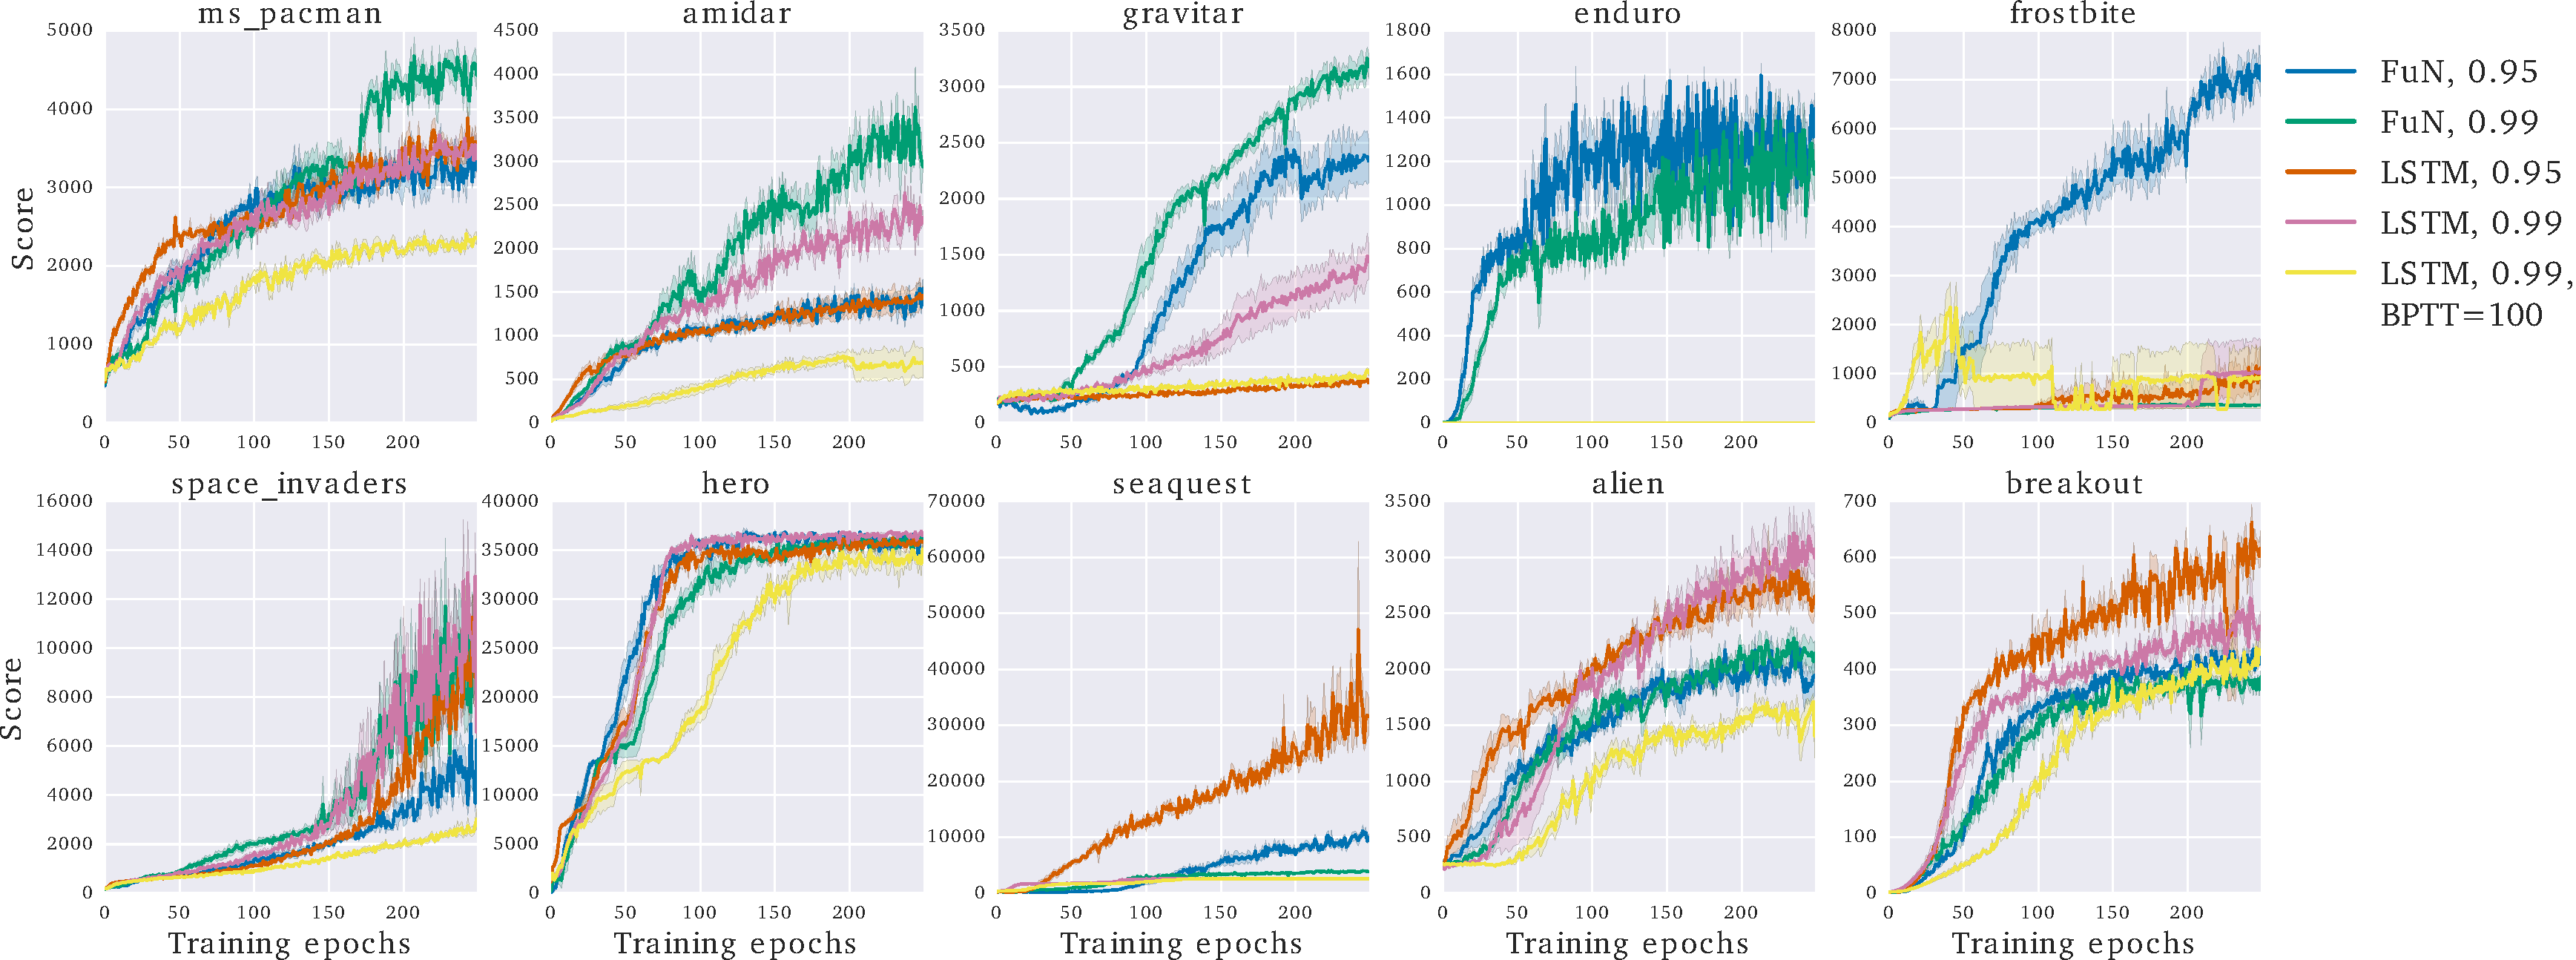
\includegraphics[scale=0.28]{./Figures/FuN_all_curves.pdf}}
  \caption{ ATARI training curves. Epochs corresponds to a million training steps of an agent. The value is the average per episode score of top 5 agents, according to the final score. We used two different discount factors $0.95$ and $0.99$. \label{fig:ATARI_all_curves} \figskiny }
\end{figure*}

\parskiny
\paragraph{Optimisation.} We use the A3C method~\cite{mnih2016asynchronous} for all reinforcement learning experiments. It was shown to achieve state-of-the-art results on several challenging benchmarks~\cite{mnih2016asynchronous}.
We cut the trajectory and run backpropagation through time (BPTT)~\cite{mozer1989focused} after $K$ forward passes of a network or if a terminal signal is received. For FuN $K=400$, for LSTM, unless otherwise stated, $K=40$. We discuss different choice of $K$ for LSTM in section~\ref{subsec:atari}.
The optimization process runs 32 asynchronous threads using shared RMSProp. There are 3 hyper-parameters in FuN and 2 in the LSTM baselines. For each method, we ran 100 experiments, each using randomly sampled hyper-parameters. Learning rate and entropy penalty were sampled from a $\mathit{LogUniform}(10^{-4},10^{-3})$ interval for LSTM. For FuN the learning rate was sampled from $\mathit{LogUniform}(10^{-4.5},10^{-3.5})$, to account for higher gradients due to longer BPTT unrolls. The learning rate was linearly annealed from a sampled value to half the initial rate for all agents. To explore intrinsic motivation in FuN, we sample its weight $\alpha \sim \mathit{Uniform}(0,1)$. We define a training epoch as one million observations.  When reporting learning curves, we plot the average episode score of the top 5 agents (according to the final score) against the training epochs. For all ATARI experiments we clip the reward to $[-1,+1]$ interval



\subseckiny
\subsection{Montezuma's revenge}
\subseckiny
\label{subsec:Montezuma}



Montezuma's revenge is one of the hardest games available through the ALE~\cite{bellemare-ale}. The game is infamous for challenging agents with lethal traps and sparse rewards.  We had to broaden and intensify our hyper-parameter search for the LSTM baseline to see any progress at all for that model. We have experimented with many different hyper-parameter configurations for LSTM baseline, for instance expanding learning rate search to $\mathit{LogUniform}(10^{-3},10^{-2})$, and we report on the configuration that worked best. We use a small discount $0.99$ for LSTM; for FuN we use $0.99$ in Worker and $0.999$ in Manager.
Figure~\ref{fig:Montezuma}b analyses the sub-goals learnt by FuN in the first room. They turn out to be meaningful milestones, which bridge the agents progress to its first extrinsic reward -- picking up the key. Interestingly, two of the learnt sub-goals correspond to roughly the same locations as the ones hand-crafted in~\cite{tejas2016hdrl} (ladder and key), but here they are learnt by the agent itself. Figure~\ref{fig:Montezuma}a plots the learning curves. Notice how FuN starts learning much earlier and achieves much higher scores. It takes $>300$ epochs for LSTM to reach the score $400$, which corresponds to solving the first room (take the key, open a door); it stagnates at that score until about $900$ epochs, when it starts exploring further. FuN solves the first room in less than $200$ epochs and immediately moves on to explore further, eventually visiting several other rooms and scoring up to $2600$ points. 


\begin{figure*}
\subfloat[]
{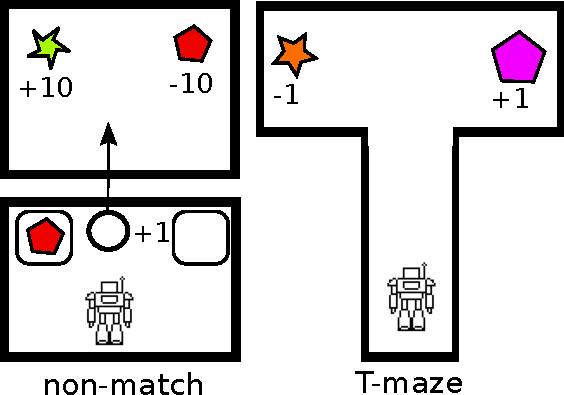
\includegraphics[scale=0.5]{./Figures/tmaze_non_match_schematics.pdf}  } 
\subfloat[]{ 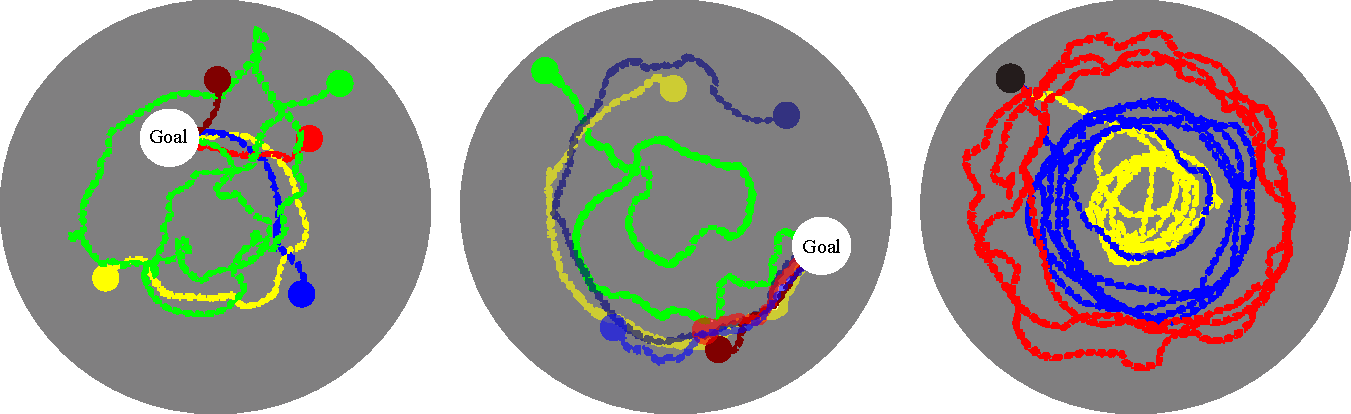
\includegraphics[scale=0.5]{./Figures/watermaze_options.pdf} }
\caption{ a) Schematic illustration of t-maze and non-match domains b) FuN in water maze. First two plots from the left, are a visualisation of FuN trajectories during one episode. The first trajectory (green) performs a search for the target in different locations, while subsequent ones (other colours) perform searches along a circle of a fixed radius matched to that of the target, always finding the target. The rightmost plot visualises different learnt sub-policies, produced by sampling a random $g$ and fixing it for 200 steps. Each colour corresponds to a different $g$, the black circle represents the starting location. \label{fig:watermaze_options} \figskiny  }
\end{figure*}


\begin{figure*}[h]
\adjustbox{trim={.05\width} {.48\height} {0.05\width} {.068\height},clip}%
{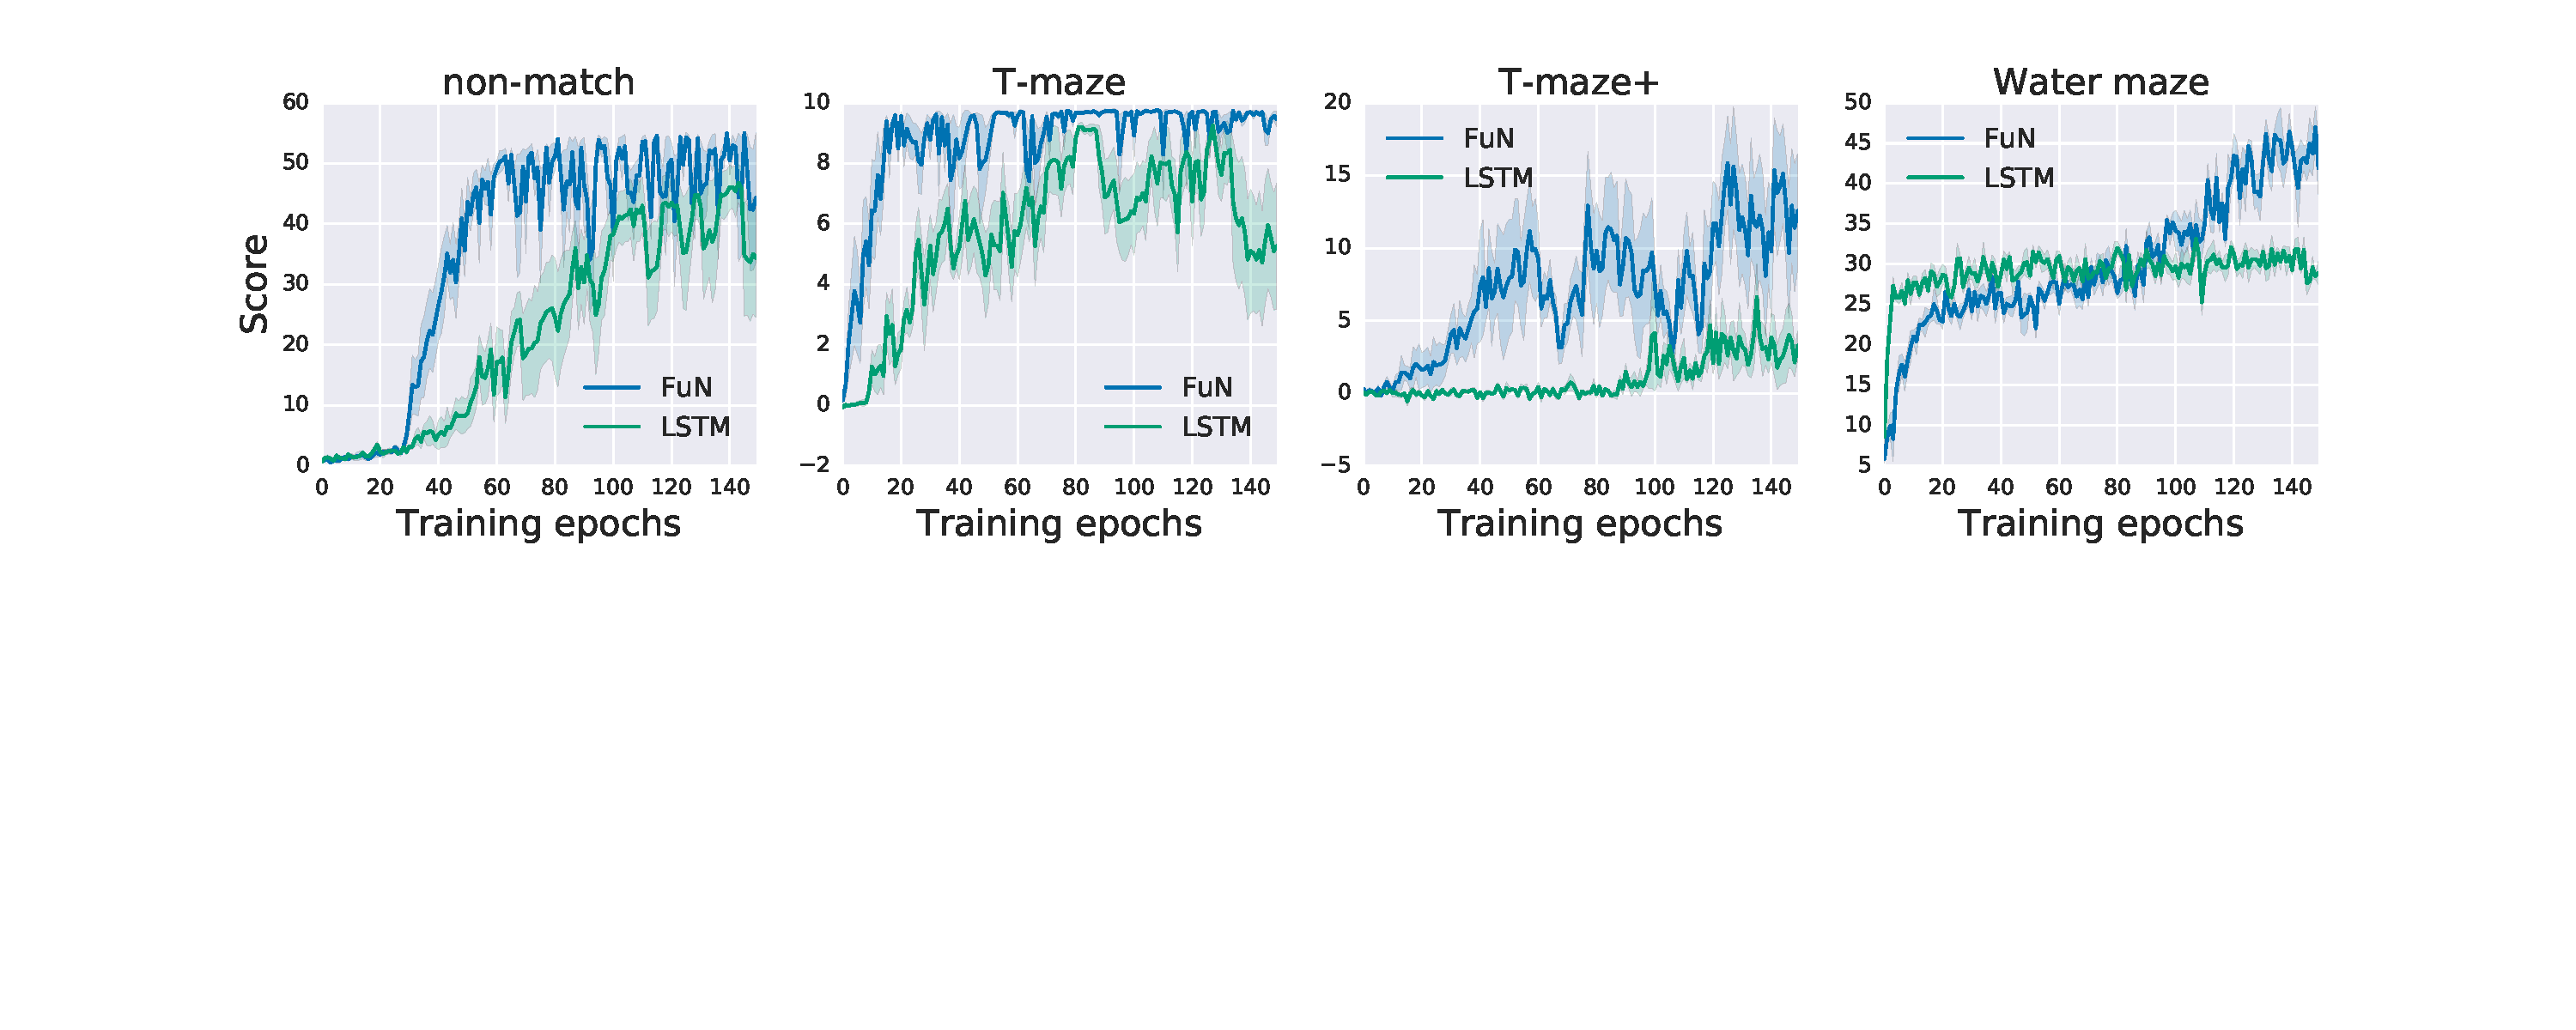
\includegraphics[scale=0.35]{./Figures/Laby_graphs.pdf}}
  \caption{ Training curves for memory tasks on Labyrinth. \label{fig:Laby_all_curves} \figskiny }
\end{figure*}

\subseckiny
\subsection{ATARI}
\subseckiny
\label{subsec:atari}

Experiments in this section validate that the capabilities of FuN go beyond what standard tools for long-term credit assignment -- discount factors and BPTT unroll length -- can provide for a baseline LSTM agent.
We use two discounts $0.99$ and $0.95$ for both FuN and LSTM agents. (For the experiments on FuN only the discount for the Manager changes, while the Worker's discount is fixed at $0.95$.) For the LSTM we explore BPTT of $40$ and $100$, while for FuN we use a BPTT unroll of $400$. For LSTM with BPTT $100$ we search for learning rate in the interval  $\mathit{LogUniform}(10^{-4.5},10^{-3.5})$, as for FuN. We use a diverse set of ATARI games, some of which involve long-term credit assignment and some which are more reactive. 

Figure~\ref{fig:ATARI_all_curves} plots the learning curves. A few categories emerge. On Ms. Pacman, Amidar, and Gravitar FuN with a low Manager discount of $0.99$ strongly outperforms all other methods. All of these games are known to require long-term reasoning to play well. Enduro stands out as all the LSTM agents completely fail at it. In this game the agent controls a racing car and scores points for overtaking other racers; this requires accelerating and steering for significant amount of time before the first reward is experienced. Frostbite is a hard game~\cite{vezhnevets2016straw, lake2016likehumans} that requires both long-term credit assignment and good exploration. The best-performing frostbite agent is FuN with $0.95$ Manager discount, which outperforms the rest by a factor of 7. On Hero and Space Invaders all agents perform equally well. 
%
On Seaquest and Breakout, the baseline LSTM with a more aggressive discount of $0.95$ is the best. This suggests that in these games long-term credit assignment is not important and the agent is better off optimising more immediate rewards in a greedy fashion. Alien is the only game where using different discounts doesn't meaningfully influence the agents performance; here we see the baseline LSTM outperforms our FuN model, although both still achieve a satisfactory scores. We provide qualitative analysis of sub-policies learnt on Seaquest in supplementary material.

Note how using an unroll for BPTT=100 in the baseline LSTM significantly hurts its performance (hence we do not explore longer unrolls), while FuN performs very well with BPTT of $400$ thanks to its ability to leverage the dLSTM. 
Being able to train a recurrent network over very long sequences could be an enabling tool for many memory related task, as we demonstrate in section~\ref{subsec:Mem_in_Lab}. 

\paragraph{Qualitative analysis on Seaquest}

To qualitatively inspect sub-policies learnt by the Worker we use the following procedure: first, we record goals emitted by Manager during the play; we then sample one of them and provide it as a constant input to the Worker for the duration of an episode and record its behaviour. This allows us to qualitatively inspect what kind of sub-policies emerge. Figure~\ref{fig:SeaQ_subgoals} plots sub-policies learnt on the seaquest game. Notice how different options correspond to rough spatial positions or manoeuvres for the agent's submarine -- for instance sub-policy 3 corresponds to swimming up for air. 


\parskiny
\paragraph{Option-critic architecture}~\cite{bacon2015option} is, to the best of our knowledge, the only other end-to-end trainable system with sub-policies. The experimental results for Option-Critic on 4  ATARI~\cite{bacon2015option} games show scores similar those from a flat DQN~\cite{mnih-dqn-2015} baseline agent. Notice that our baseline~\cite{mnih2016asynchronous} is much stronger than DQN. We also ran FuN on the same games as Option-Critic (Asterix, Ms. Pacman, Seaquest and Zaxxon) and after 200 epochs it achieves a similar score on Seaquest, doubles it on Ms. Pacman, more than triples it on Zaxxon and gets more than 20x improvement on Asterix.  Figure~\ref{fig:OptCrit} presents our results on Asterix and Zaxxon. We took the approximate performance of Option-Critic from the original paper -- 8000 for Asterix and 6000 for Zaxxon. Plots in the original paper also suggest that score stagnates around these levels, notice that our score keeps going up.

\begin{figure}[h]
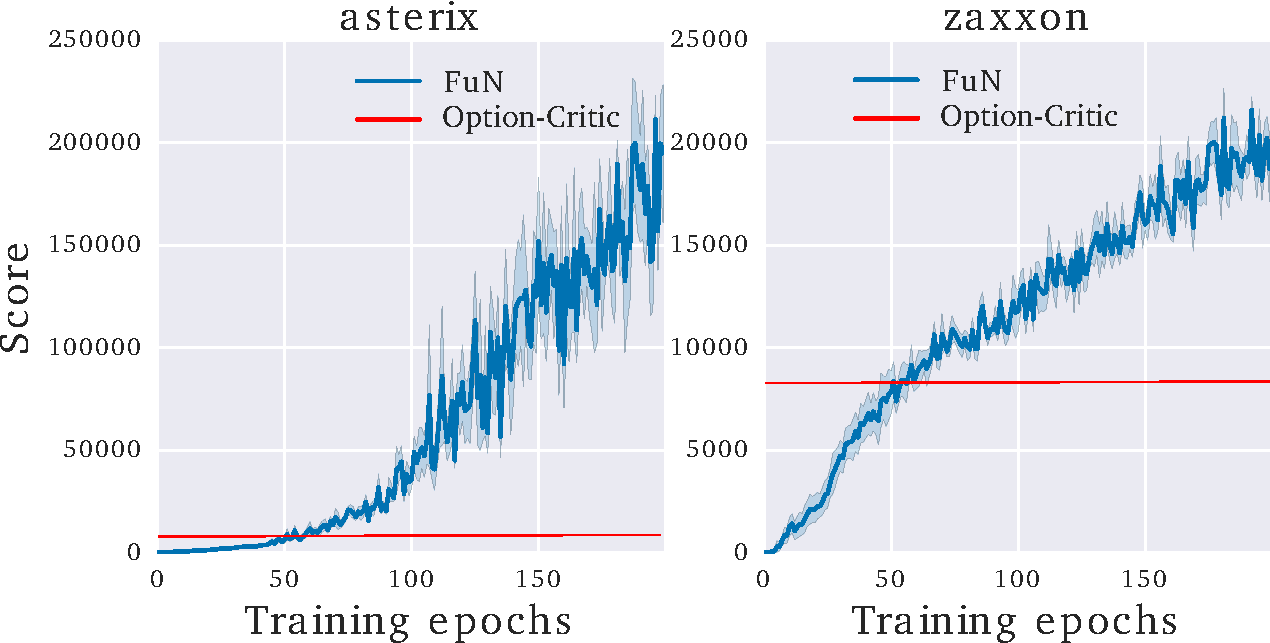
\includegraphics[scale=0.35]{./Figures/VsOptCrit.pdf}
  \caption{Comparison to Option-Critic on Zaxxon and Asterix. Score for Option-Critic is taken from the original paper  \label{fig:OptCrit} \figskiny }
\end{figure}


\begin{figure*}[h]
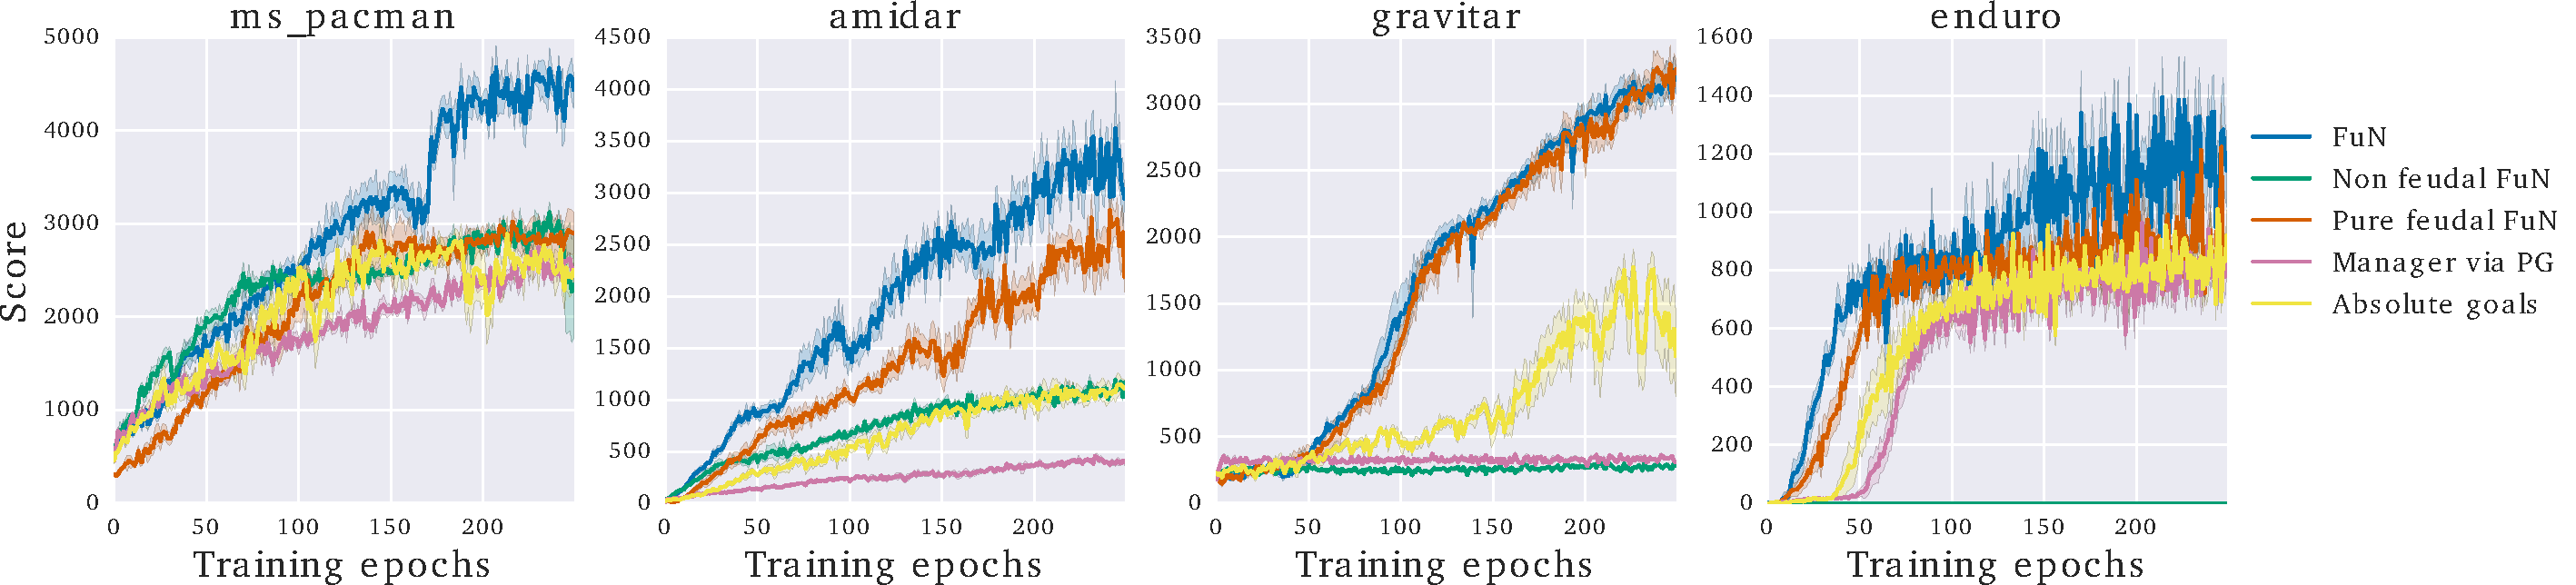
\includegraphics[scale=0.35]{./Figures/Ablation_curves.pdf}
  \caption{ Ablative analysis \label{fig:Ablation_curves} }
\end{figure*}

\begin{figure*}[h]
{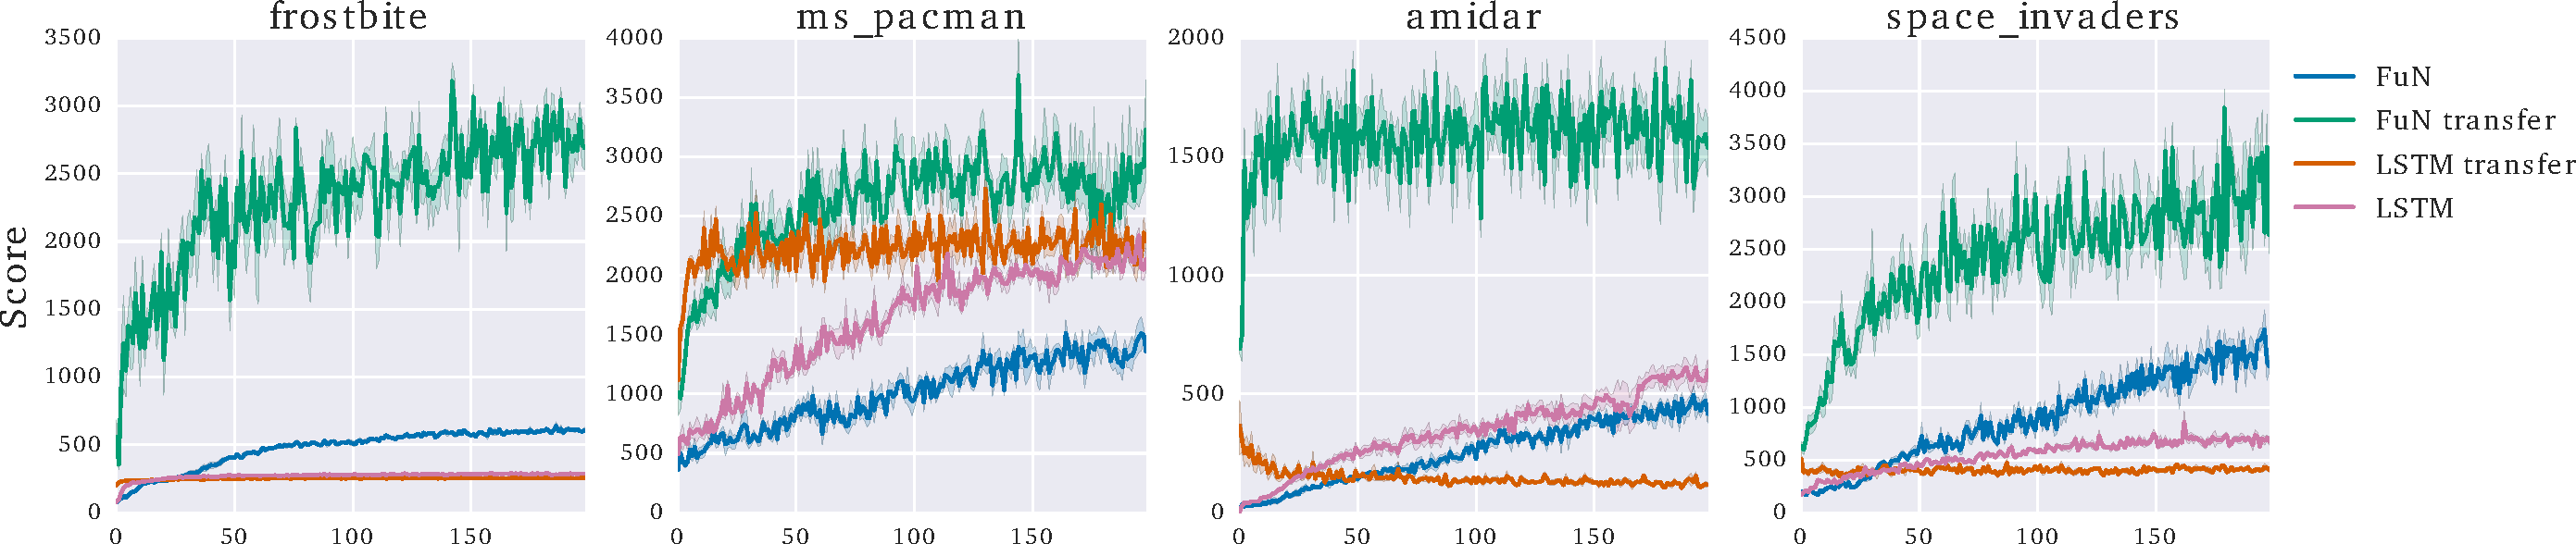
\includegraphics[scale=0.35]{./Figures/ActRep_graphs.pdf}}
  \caption{ Action repeat transfer \label{fig:ActRep_graphs} \figskiny }
\end{figure*}

\subseckiny
\subsection{Memory in Labyrinth}
\subseckiny
\label{subsec:Mem_in_Lab}
DeepMind Lab~\cite{beattie2016labyrinth} is a first-person 3D game platform extended from OpenArena. It's a visually complex 3D environment with agent actions corresponding to movement and orientation. We use 4 different levels that test long-term credit assignment and visual memory: 

\parskiny
\paragraph{Water maze} is a reproduction of the Morris water maze experiment~\cite{morris1981watermaze} from the behavioural science literature. An agent is dropped into a circular pool of water with a concealed platform at unknown random location. The agent can move around and upon stepping on the platform it receives a reward and the trial restarts. The platform remains in the same location for the rest of the episode, while agent starts each trial at a random location. The walls of the pool are decorated with visual cues to assist localisation. 

\parskiny
\paragraph{T-maze} is another classic animal cognition test. The agent spawns in a small T-shaped maze.  Two objects with randomly chosen shape and colour are spawned at the left and right "baiting" locations.  One of them is assigned a reward of +1 and the other a reward of -1.  When the agent collects one of the objects, it receives the reward and is re-spawned at the beginning of the T-maze. The objects are also re-instantiated in the same locations and with the same rewards on the re-spawn event. The agent should remember which object gives the positive reward across re-spawns and collect it as many times as possible within the fixed time given for the episode. \textbf{T-maze+} is a modification of T-maze, where at each trial the length of corridors can vary, adding additional dimension of complexity. 

\parskiny
\paragraph{Non-match} is a visual memorisation task. Each trial begins in small room with an out of reach object being displayed in one of two display pods. There is a pad in the middle, which upon touching, the agent is rewarded with 1 point, and is teleported to a second room which has two objects in it, one of which matches the object in the previous room. Collecting the matching object gives a reward of -10 points, collecting the non matching object gives a reward of 10 points. Once either is collected, the agent is teleported back to the first room, with the same object being shown.

For all agents we include reward as a part of the observation.
Figure~\ref{fig:watermaze_options}a illustrates T-maze and non-match environments and 
figure~\ref{fig:Laby_all_curves} plots the learning curves. FuN consitently outperforms the LSTM baseline -- it learns faster and also reaches a higher final reward. We analyse the FuN agent's behaviour in more detail in Figure~\ref{fig:watermaze_options}b. It demonstrates that FuN learns meaningful sub-policies, which are then efficiently integrated with memory to produce rewarding behaviour. Interestingly, the LSTM agent doesn't appear to use its memory for water maze task at all, always circling the maze at the roughly the same radius. 

\subseckiny
\subsection{Ablative analysis}
\subseckiny
\label{subsec:ablative}


This section empirically validates the main innovations of this paper: transition policy gradient for training the Manager; relative rather than absolute goals; lower temporal resolution for Manager; intrinsic motivation for the Worker.

\paragraph{Transition policy gradient} First we consider a `non-Feudal' FuN -- it has exactly the same network architecture as FuN, but the Manager’s output $g$ is trained with gradients coming directly from the Worker and no intrinsic reward is used, much like in Option-Critic architecture~\cite{bacon2015option}.  Second, $g$ is learnt using a standard policy gradient approach with the Manager emitting the mean of a Gaussian distribution from which goals are sampled (as if the Manager were solving a continuous control problem~\cite{schulman2015gae,mnih2016asynchronous,lillicrap2015continuous}). Third, we explore a variant of FuN in which $g$ specifies absolute, rather than relative/directional, goals (and the Worker's intrinsic reward is adjusted accordingly) but otherwise everything is the same.
The experiments (Figure~\ref{fig:Ablation_curves}) reveal that, although alternatives do work to some degree their performance is significantly inferior. We also evaluate a purely feudal version of FuN -- in which the Worker is trained from the intrinsic reward alone. This ablation performs better than other, but still inferior to the full FuN approach. It shows that allowing the Worker to experience the external reward is beneficial. 

\paragraph{Temporal resolution ablations.}  An important feature of FuN is the ability of the Manager to operate at a low temporal resolution. This is achieved through dilation in the LSTM and through the prediction horizon $c$. To investigate their influence we use two baselines:
i) the Manager uses a vanilla LSTM with no dilation; ii) FuN with Manager's prediction horizon $c=1$. Figure~\ref{fig:ablation_temp} presents the results. The non-dilated LSTM fails catastrophically, most likely overwhelmed by the recurrent gradient. Reducing the horizon $c$ to 1 did hurt the performance, although interestingly less so than other ablations. It seems that even at high temporal resolution Manager captures certain properties of the underlying MDP and communicate them down to Worker in a helpful way. This confirms that by learning in two separate formulations FuN is able to capture richer structural properties of the environment and thus train faster. 

\begin{figure*}[h!]
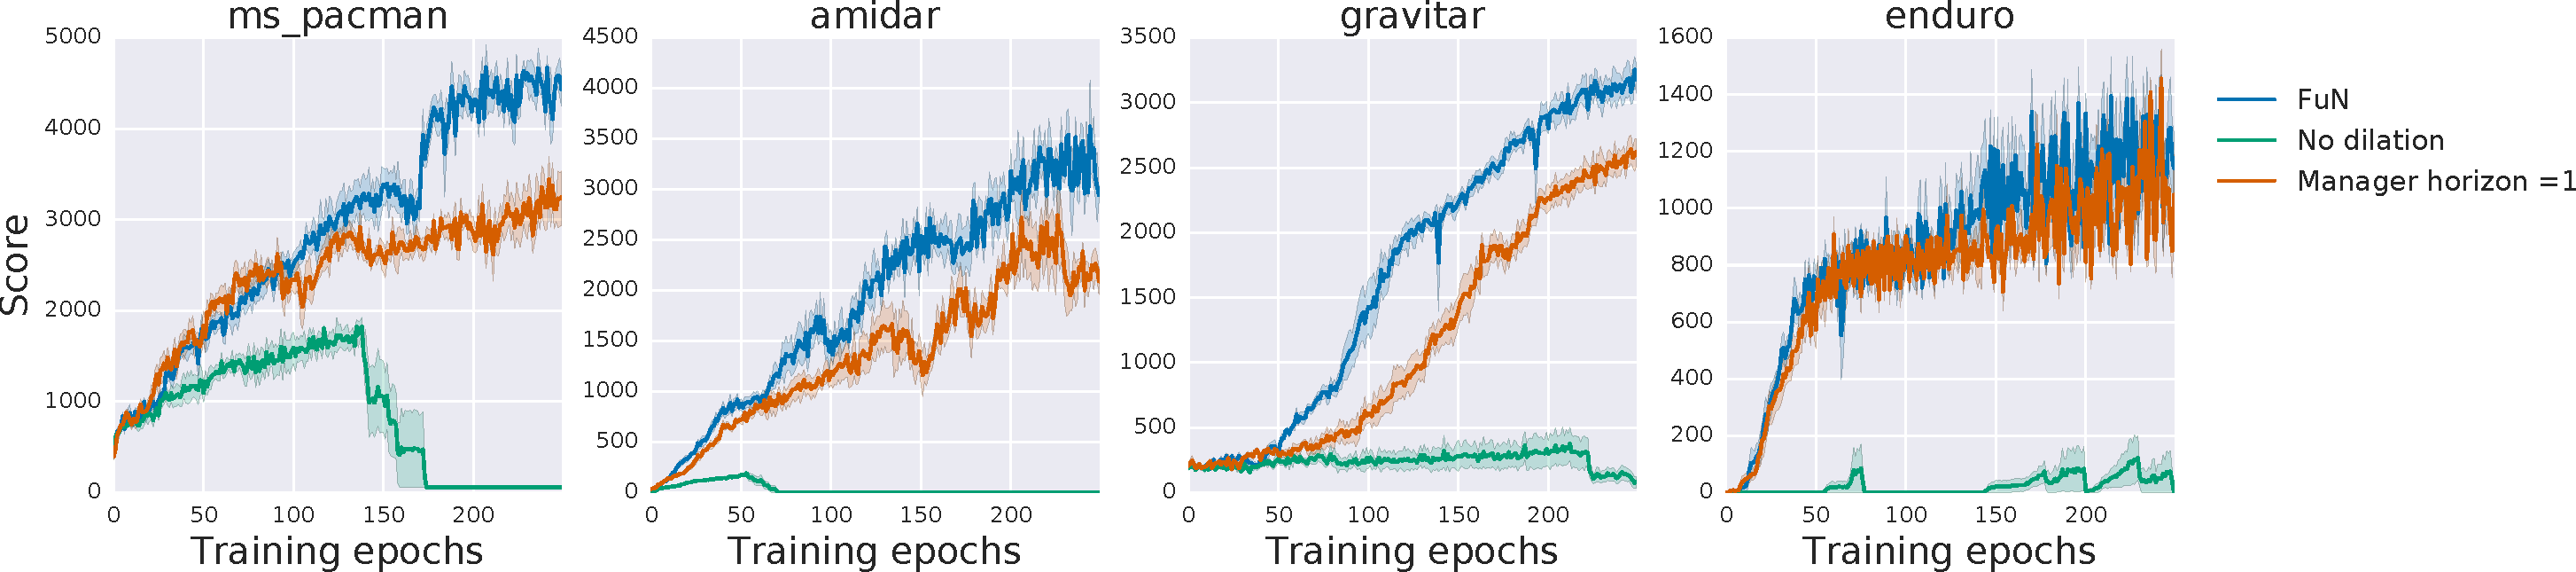
\includegraphics[scale=0.35]{./Figures/Ablation_temp_curves.pdf}
  \caption{ Learning curves for ablations of FuN that investigate influence of dLSTM in the Manager and Managers prediction horizon $c$. No dilation -- FuN trained with a regular LSTM in the Manager; Manager horizon =1 -- FuN trained with $c=1$.\label{fig:ablation_temp} \figskiny }
\end{figure*}

\begin{figure*}[h!]
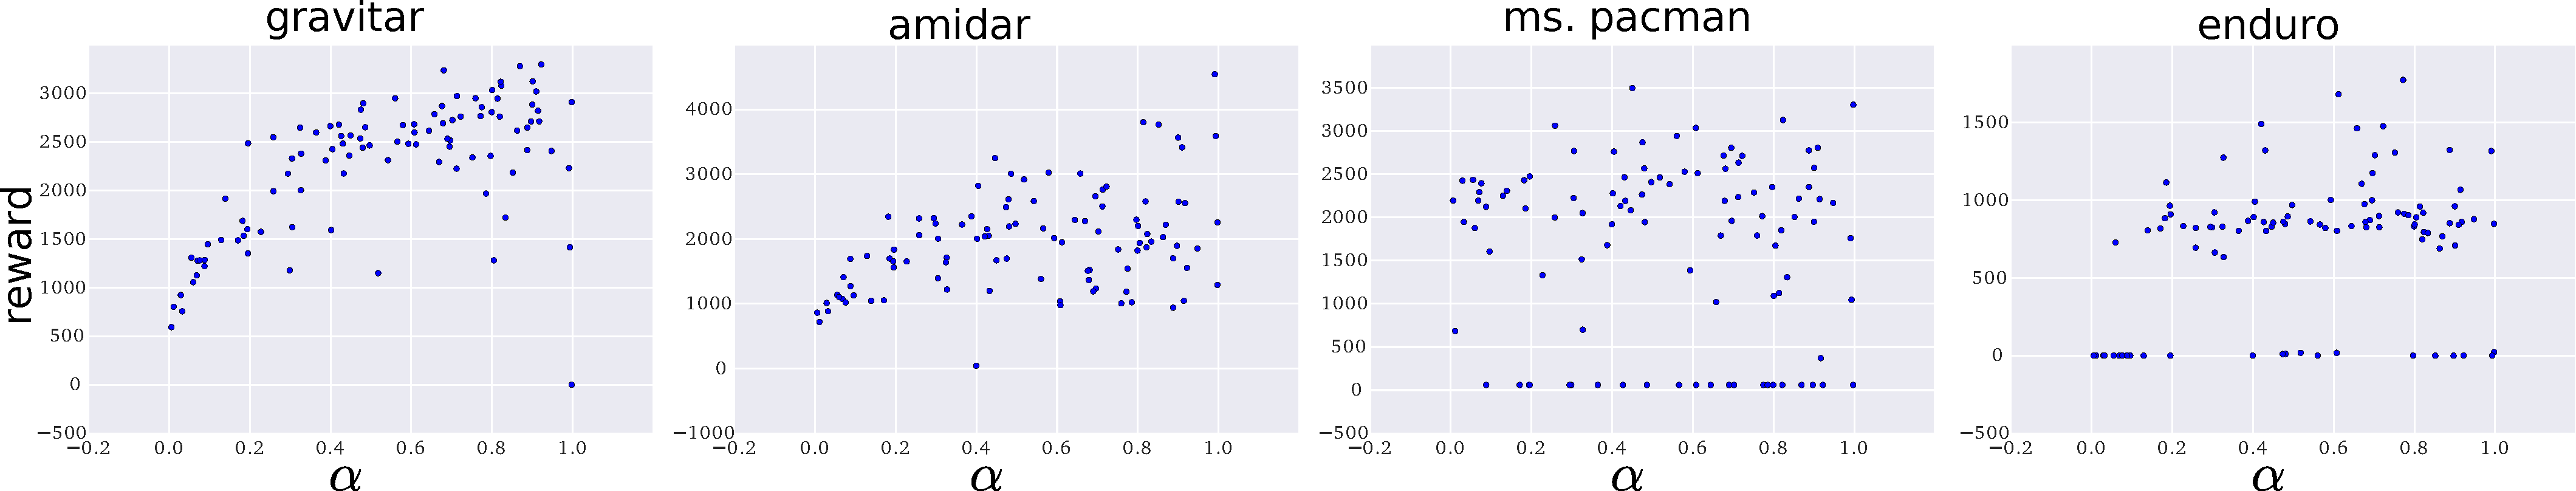
\includegraphics[scale=0.22]{./Figures/alpha_scatter_plots.pdf}
  \caption{Scatter plot of agents reward after $200$ epochs vs intrinsic reward weight $\alpha$. \label{fig:alpha_scatter_plots} \figskiny }
\end{figure*}

\paragraph{Intrinsic motivation weight.} This section look at the impact of the weight $\alpha$, which regulates the relative weight of intrinsic reward (if $\alpha=0$ then intrinsic reward is not used). We train agents with learning rate and entropy penalty fixed to $10^{-3.5}$ and only vary $\alpha$ between $[0,1]$. Figure~\ref{fig:alpha_scatter_plots} shows scatter plots of agent’s final score vs $\alpha$ hyper-parameter.  Notice a clear correlation between the score and high value of $\alpha$ on gravitar and amidar; however on other games the optimal value of $\alpha$ can be less than to $1$.

\paragraph{Dilate LSTM agent baseline}
One of innovations this paper presents is dLSTM design for a Recurrent network. In principle, it could alone be used in an agent on top of a CNN, without the rest of FuN structures. We evaluate such an agent as an additional baseline. We use the same hyper-parameters as for FuN -- BPTT=400, discount $=0.99$, learning rate sampled in the interval $\mathit{LogUniform}(10^{-4.5},10^{-3.5})$, entropy penalty $\mathit{LogUniform}(10^{-4},10^{-3})$. Figure~\ref{fig:dLSTM_curves} plots the learning curves for FuN, LSTM and dLSTM agents. dLSTM generally underperforms both LSTM and FuN. The power of dLSTM is in the ability to operate at lower temporal resolution, which is useful in the Manager, but not so much on it's own.

\begin{figure*}[h!]
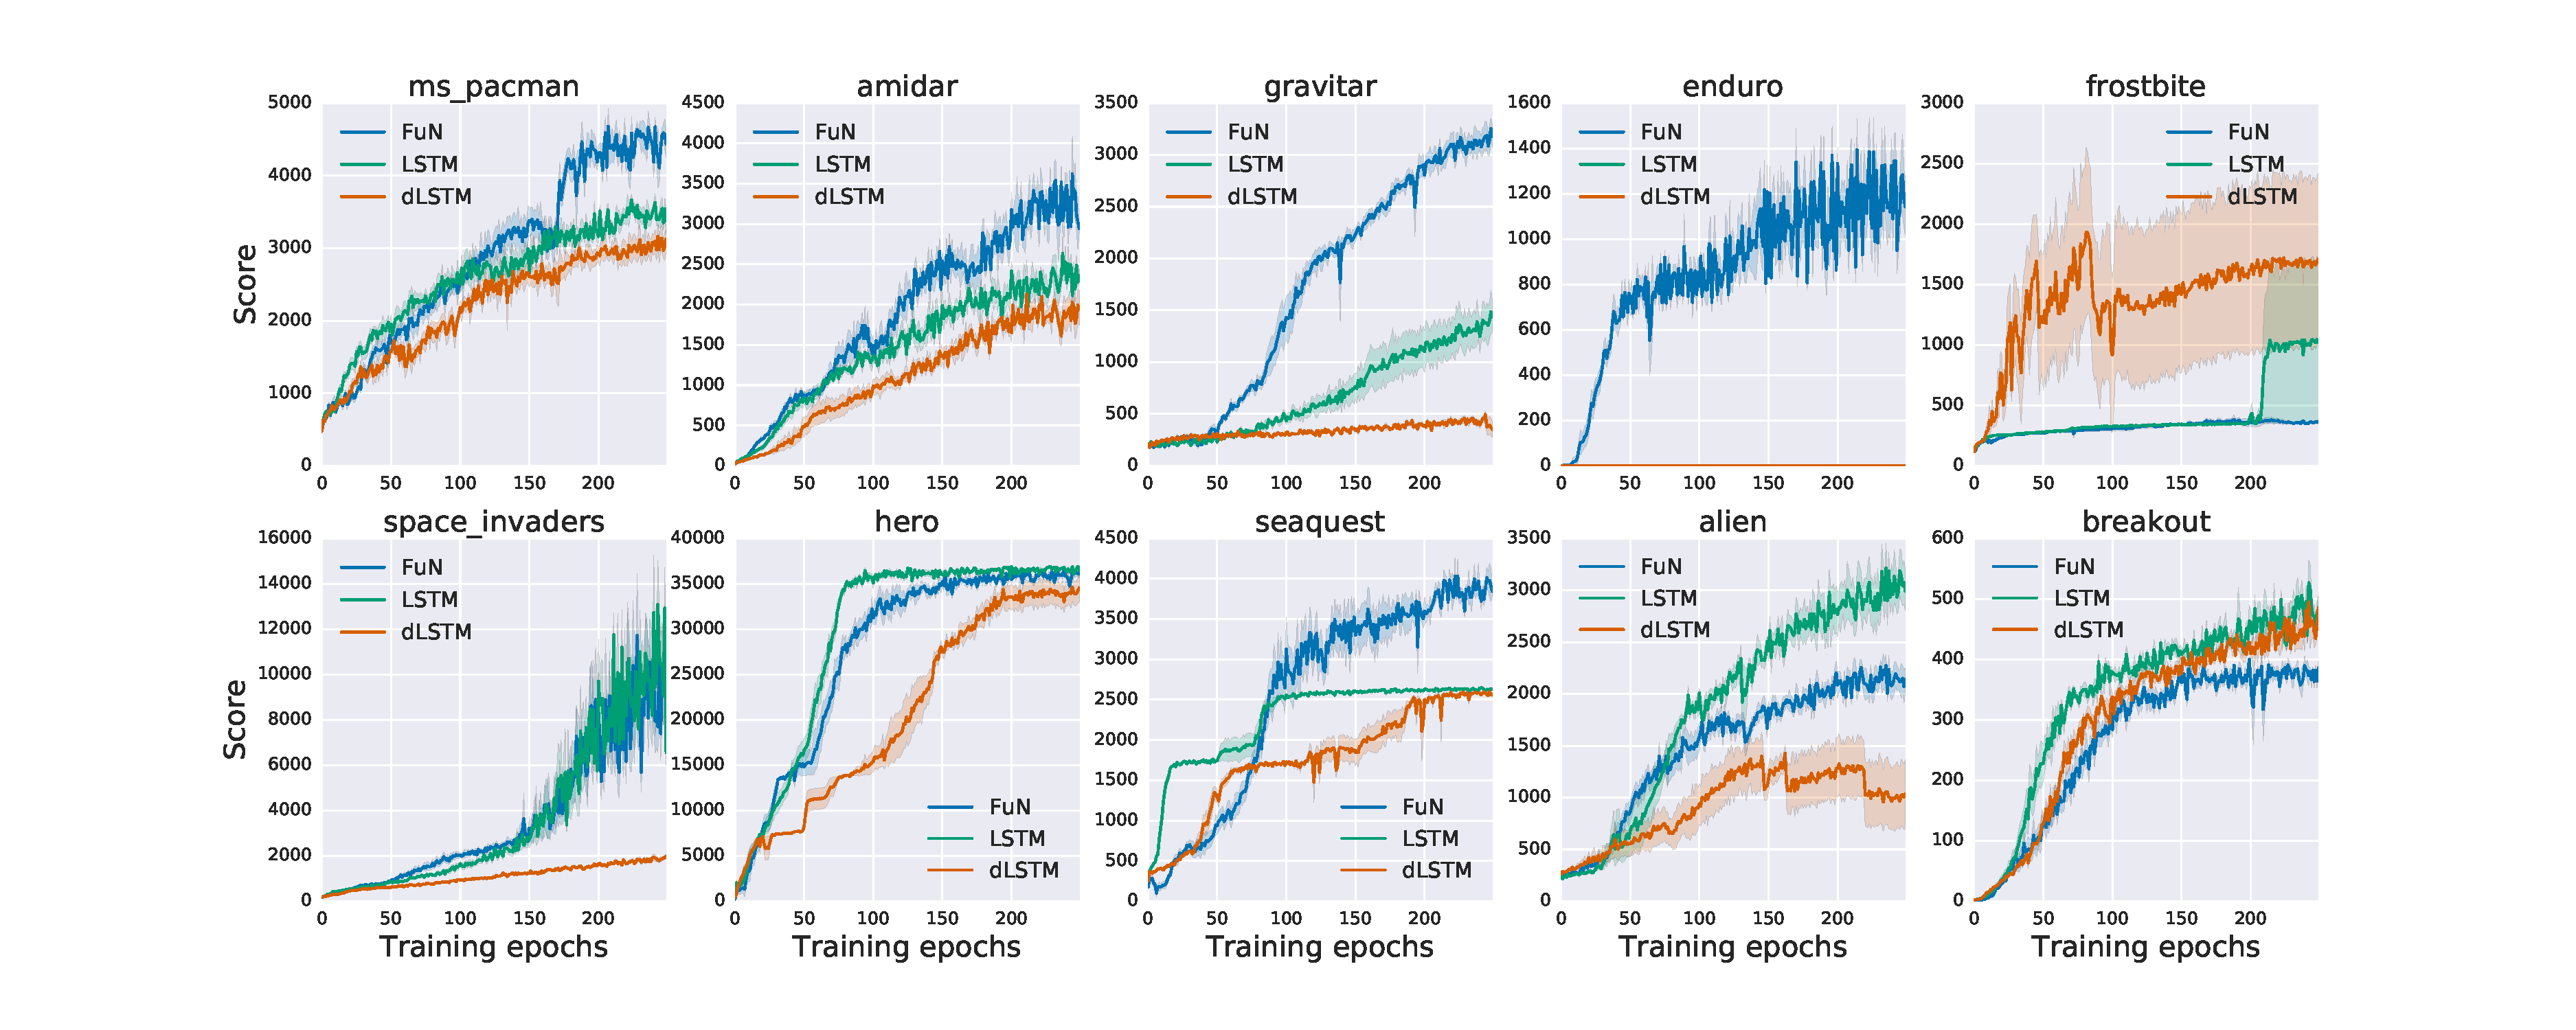
\includegraphics[scale=0.25]{./Figures/dLSTM_all_curves.pdf}
  \caption{Learning curves for dLSTM based agent with LSTM and FuN for comparison. \label{fig:dLSTM_curves} \figskiny }
\end{figure*}


\subseckiny
\subsection{ATARI action repeat transfer}
\subseckiny
One of the advantages of FuN is the clear separation of duties between Manager and Worker. The Manager learns a transition policy, while the Worker learns to operate primitive actions to enact these transitions. This transition policy is invariant to the underlying embodiment of the agent -- the way its primitive actions translate into state space transitions. Potentially, the transition policy can be transferred between agents with different embodiment -- e.g. robot models with physical design or different operational frequency. We provide evidence towards that possibility by transferring policies across agents with different action repeat on ATARI.\footnote{Action repeat is a heuristic used in all successful agents~\cite{mnih-dqn-2015, mnih2016asynchronous, bellemare2016gap, vezhnevets2016straw}. It enables better exploration, eases credit assignment, and saves computation by repeating any action chosen by the agent several ($=4$) times.}


To perform transfer, we initialise the FuN system with parameters extracted from an agent trained with action repeat of $4$ and then make the following adjustments: (i) we accordingly adjust the discounts for all rewards; (ii) we increase the dilation of the dLSTM by a factor of 4; (iii) we increase the Manager's goal horizon $c$ by a factor of 4. (These modifications adapt all the ``hard-wired'' but explicitly temporally sensitive aspects of the agent.) We then train this agent without action repeat. As a baseline we use an LSTM agent transferred in a similar way (with adjusted discounts) as well as FuN and LSTM agents trained without action repeat from scratch. Figure~\ref{fig:ActRep_graphs} shows the corresponding learning curves. The transferred FuN agent (green curve) significantly outperforms every other method. Furthermore it shows positive transfer on each environment, whereas LSTM only shows positive transfer on Ms. Pacman.


